%
% CSE Electronic Homework Template
% Last modified 8/23/2018 by Jeremy Buhler

\documentclass[11pt]{article}
\usepackage[left=0.7in,right=0.7in,top=1in,bottom=0.7in]{geometry}
\usepackage{fancyhdr} % for header
\usepackage{graphicx} % for figures
\usepackage{amsmath}  % for extended math markup
\usepackage{amssymb}
\usepackage[bookmarks=false]{hyperref} % for URL embedding
\usepackage[noend]{algpseudocode} % for pseudocode
\usepackage[plain]{algorithm} % float environment for algorithms

%%%%%%%%%%%%%%%%%%%%%%%%%%%%%%%%%%%%%%%%%%%%%%%%%%%%%%%%%%%%%%%%%%%%%%
% STUDENT: modify the following fields to reflect your
% name/ID, the current homework, and the current problem number

% Example: 
%\newcommand{\StudentName}{Jeremy Buhler}
%\newcommand{\StudentID{123456}

\newcommand{\StudentName}{Dingyu Wang (Howard)}
\newcommand{\StudentID}{COMP 642: Machine Learning}
\newcommand{\HomeworkNumber}{4}

%%%%%%%%%%%%%%%%%%%%%%%%%%%%%%%%%%%%%%%%%%%%%%%%%%%%%%%%%%%%%%%%%%%%%%%%
% You can pretty much leave the stuff up to the next line of %%'s alone.

% create header and footer for every page
\pagestyle{fancy}
\fancyhf{}
\lhead{\textbf{\StudentName}}
\chead{\textbf{\StudentID}}
\rhead{\textbf{HW \HomeworkNumber}}
\cfoot{\thepage}

% preferred pseudocode style
\algrenewcommand{\algorithmicprocedure}{}
\algrenewcommand{\algorithmicthen}{}

% ``do { ... } while (cond)''
\algdef{SE}[DOWHILE]{Do}{doWhile}{\algorithmicdo}[1]{\algorithmicwhile\ #1}%

% ``for (x in y ... z)''
\newcommand{\ForRange}[3]{\For{#1 \textbf{in} #2 \ \ldots \ #3}}

% these are common math formatting commands that aren't defined by default
\newcommand{\union}{\cup}
\newcommand{\isect}{\cap}
\newcommand{\ceil}[1]{\ensuremath \left\lceil #1 \right\rceil}
\newcommand{\floor}[1]{\ensuremath \left\lfloor #1 \right\rfloor}

%%%%%%%%%%%%%%%%%%%%%%%%%%%%%%%%%%%%%%%%%%%%%%%%%%%%%%%%%%%%%%%%%%%%%%
\usepackage[utf8]{inputenc}
\usepackage[english]{babel}
\setlength{\parindent}{0em}
\setlength{\parskip}{1em}
 \usepackage{pythonhighlight}
\usepackage{graphicx}
\graphicspath{ {./images/} }


\begin{document}

% STUDENT: Your text goes here!
1) KNN \\
a) The answer is ii). We should calculate the mean and standard deviation of the training set, and apply those numbers based on the training set to both sets. We do not want to use the whole data (that includes the test set) to get the mean and standard deviation because that is introducing unseen information. We also don't want to separately use the mean and standard deviation from the test set because we don't want to create relationship between the test set. We should view it as we can only see one test data point at a time.

b) The value of k is k = 10. We can find counterexamples for k = 1 because there are blue points in the orange region and that area is all classified as orange, so definitely not 1. Similarly for k = 2, we can see there are groups of orange points, for example there are is a group of orange points in the blue area where the area is still all classified as blue. We find that for k = 10, there is no counterexample. Therefore, we conclude that k = 10. k = 100 is too large. 

c) (Executing the command to get the data. Nothing to solve.)

d) \\ \\
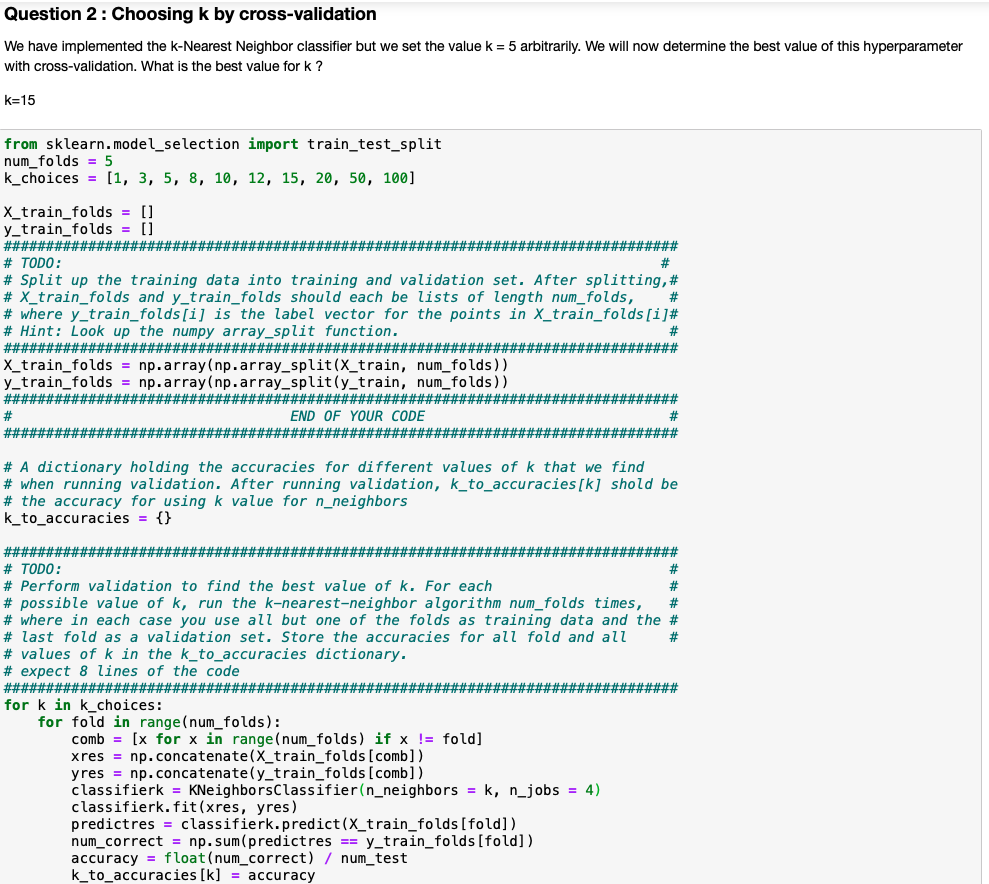
\includegraphics[scale=0.33]{knn1} \\ \\
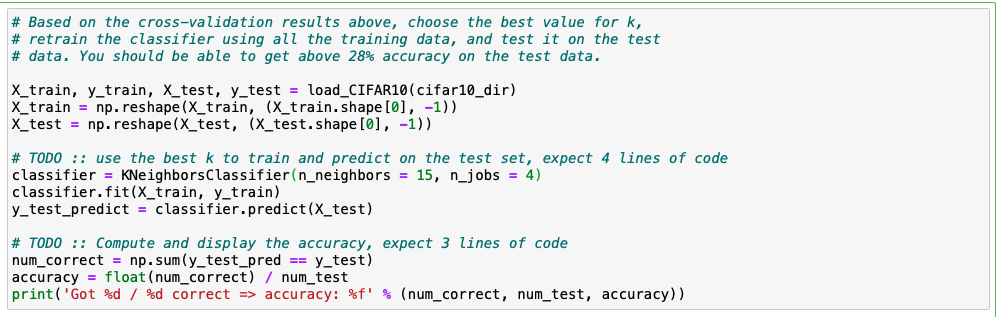
\includegraphics[scale=0.33]{knn2}

2) Decision Tree \\
a) \\
cost(D) = 400/800 = 1/2

Model A: \\
cost(D\_left) = 100/400 = 1/4 \\
cost(D\_right) = 100/400 = 1/4 \\
Reduction(D) = 1/2 - (1/2*1/4+1/2*1/4) = 1/4

Model B: \\ 
cost(D\_left) = 200/600 = 1/3 \\
cost(D\_right) =  0/200 = 0 \\
Reduction(D) = 1/2 - (3/4*1/3 + 0) = 1/4 

According to the calculations, both models are the same. \\

b)  \\
Entropy 

cost(D) = -(400/800)log\_2(400/800)-(1-400/800)log\_2(1-400/800) = 1

Model A: \\
cost(D\_left) =  -(300/400)log\_2(300/400)-(100/400)log\_2(100/400) = 0.811 \\
cost(D\_right) =  -(100/400)log\_2(100/400)-(300/400)log\_2(300/400) = 0.811 \\
Reduction(D) = 1 - (1/2*0.811+1/2*0.811) = 0.189 

Model B: \\ 
cost(D\_left) = -(200/600)log\_2(200/600)-(400/600)log\_2(400/600) = 0.918 \\
cost(D\_right) = -(200/200)log\_2(200/200)-(0)log\_2(0) = 0\\
Reduction(D) = 1-(600/800*0.918+0) = 0.3115 

Preferred split is model B.

c) \\
Gini Index 

cost(D) = 2(400/800)(400/800) = 1/2

Model A: \\
cost(D\_left) =  2(300/400)(1-300/400) = 0.375\\
cost(D\_right) =  2(100/400)(1-100/400) = 0.375\\
Reduction(D) = 1/2-(1/2*0.375+1/2*0.375) = 0.125

Model B: \\ 
cost(D\_left) = 2(200/600)(1-200/600) = 0.444\\
cost(D\_right) = 2(200/200)(1-200/200) = 0\\
Reduction(D) = 1/2-(600/800*0.444+0) = 0.167

Preferred split is model B. \\ \\
 
 
d) \\ \\
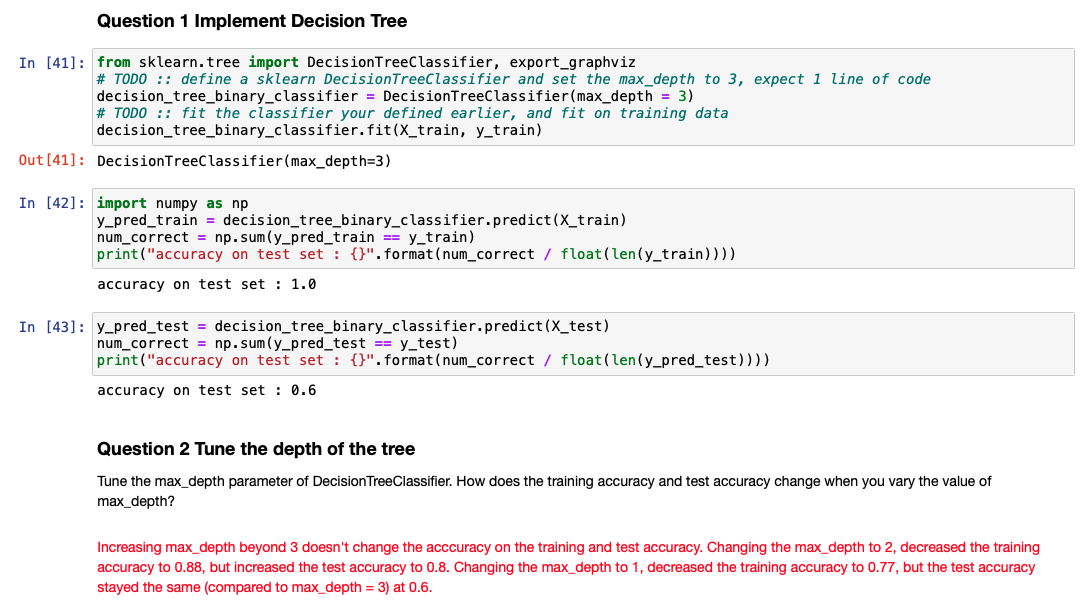
\includegraphics[scale=0.33]{decision1}

3) SVM \\ 
a) \\
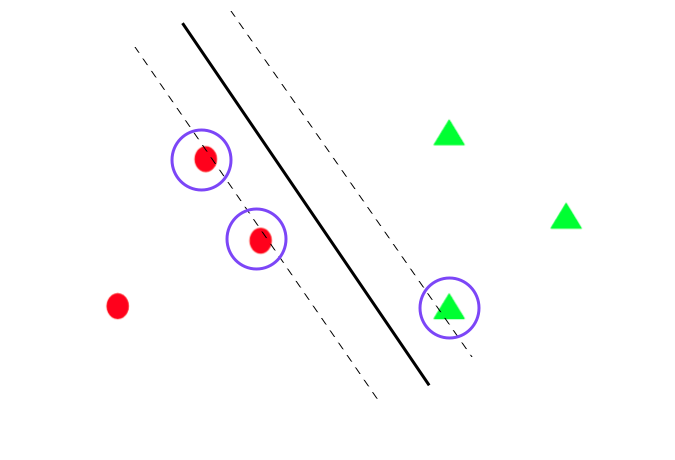
\includegraphics[scale=0.33]{drawsvm} \\ \\ 
b) \\
Yes, changing the support vectors will change the margins thus changing the decision boundary. Changing the non support vectors points when they are not at boundary does not change the support vectors. \\  \\ 
c) (next page)\\ \\
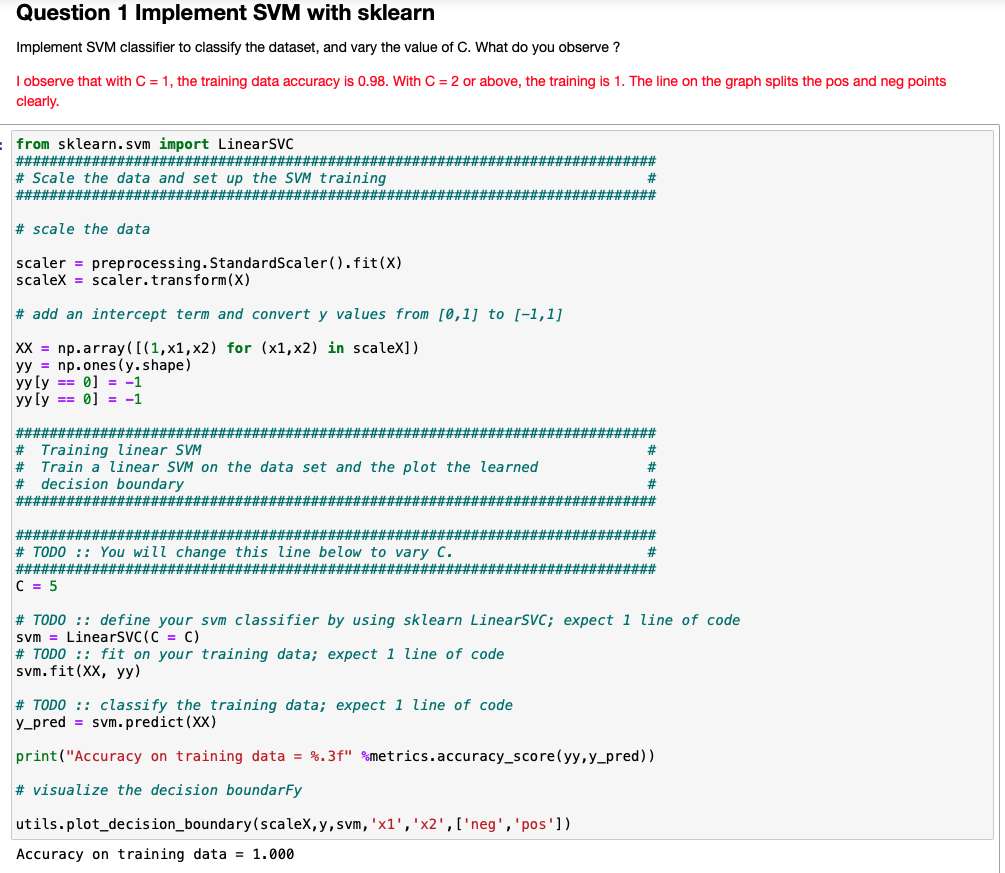
\includegraphics[scale=0.33]{svm1} \\ \\
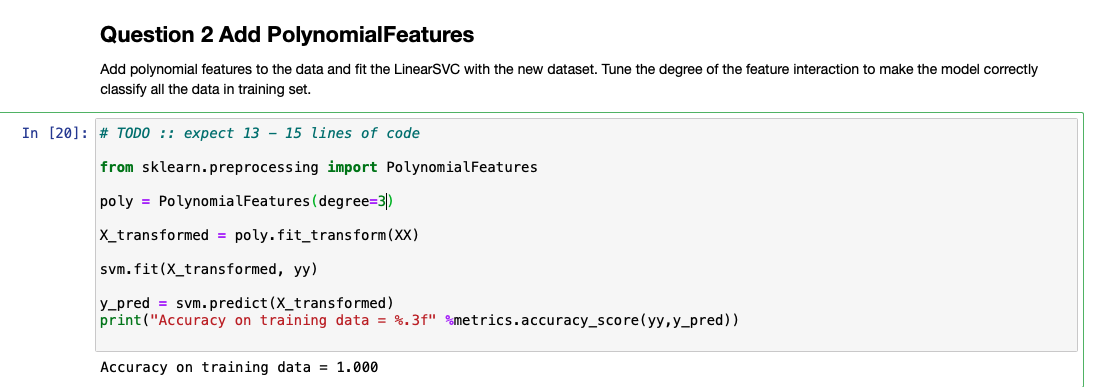
\includegraphics[scale=0.33]{svm2}

\end{document}
